\documentclass[../TDTM3.tex]{subfiles}%

\begin{document}
\section[s]"1"{Étude d'un mélange stœchiométrique}
\enonce{%
	On étudie à \SI{25}{\degreeCelsius} l'action d'une solution de soude diluée sur
	le bromoéthane~; la réaction totale a pour équation~:
	\[\ce{CH3CH2Br + HO^{-} -> CH3CH2OH + Br^{-}}\]
	On utilise des mélanges stœchiométriques en bromoéthane et en ion hydroxyde.
	Soit $c_0$ la concentration initiale commune des deux réactifs. Le tableau
	ci-dessous donne les temps de demi-réaction pour différentes valeurs de $c_0$.
	\begin{center}
		\begin{tabular}{lccccc}
			\toprule
			$c_0 (\si{mmol.L^{-1}})$ &
			10                       & 25  & 50  & 75  & 100 \\
			\midrule
			$\tau_{1/2} (\si{min})$  &
			1100                     & 445 & 220 & 150 & 110 \\
			\bottomrule
		\end{tabular}
	\end{center}
}

\QR{%
	Démontrer que ces données sont compatibles avec une réaction d'ordre
	partiel 1 par rapport à chacun des réactifs.
}{%
	Si la réaction est d'ordre 1 par rapport à chacun des réactifs, cela
	veut dire qu'elle s'écrit
	\[v = k [\ce{CH3CH2Br}][\ce{HO-}]\]
	Leurs coefficients stœchiométriques sont égaux à -1, ce qui veut dire
	que chacun de ces réactifs a une concentration $c(t) = c_0 - x(t)$ à
	chaque instant~; ainsi
	\[v = k c(t)^2\]
	Cette réaction est équivalente à une réaction d'ordre 2 par rapport à un
	unique réactif, dont le temps de demi-réaction est
	\[\tau_{1/2} = \frac{1}{kc_0}\]
	Pour vérifier que les données sont compatibles avec cette relation, on
	trace $\tau_{1/2} = f(1/c_0)$ en traçant
	\[y = ax
		\qavec
		\left\{
		\begin{array}{rcl}
			y & = & t_{1/2} \\
			a & = & 1/k     \\
			x & = & 1/c_0
		\end{array}
		\right.
	\]
	\begin{minipage}{0.45\linewidth}
		On trouve bien ici une droite avec un coefficient de corrélation
		$r^2 = \num{0.99997}$, confirmant que l'\textbf{ordre global} est
		compatible avec 2.
		\begin{tcn}(impo){Attention}
			Cette démarche ne prouve en rien que les ordres partiels sont
			chacun de 1~: ils pourraient être de 1/2 et 3/2 respectivement.
		\end{tcn}
	\end{minipage}
	\hfill
	\begin{minipage}{0.55\linewidth}
		\begin{center}
			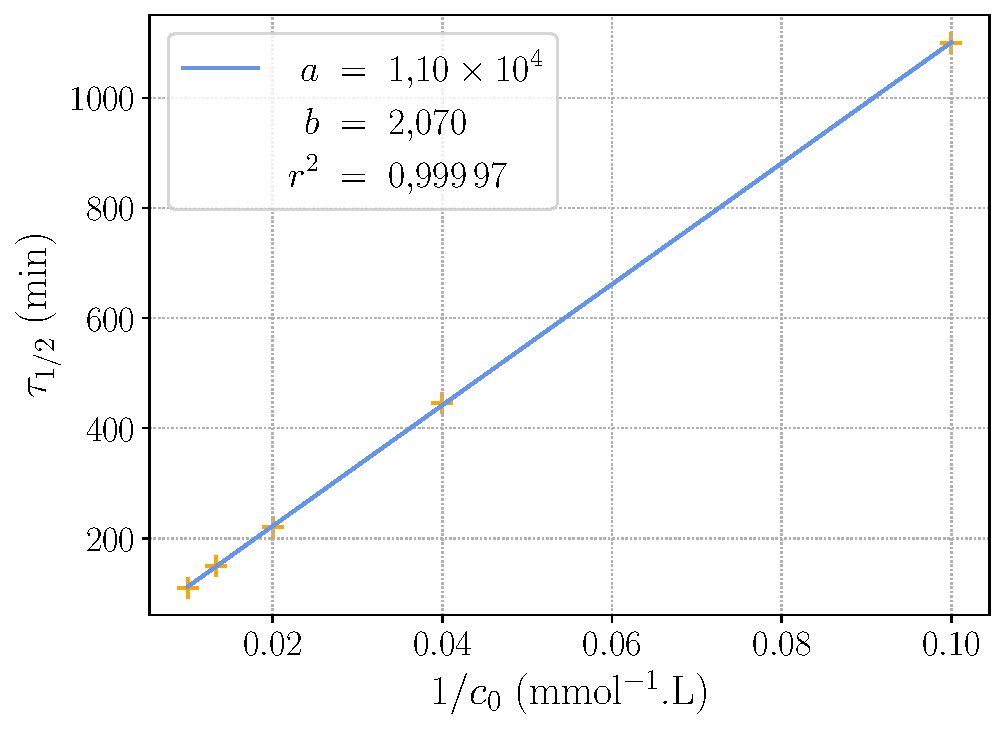
\includegraphics[width=\linewidth]{exo4_tab}
		\end{center}
	\end{minipage}
}

\QR{%
Déterminer la constante de vitesse de la réaction.
}{%
Comme déterminé dans la régression linéaire, le coefficient directeur
de la droite est l'inverse de la constante de vitesse. On trouve donc
\[\boxed{k = \SI{9.10e-5}{mmol^{-1}.L.min^{-1}} =
	\SI{9.10e-2}{mol^{-1}.L.min^{-1}}}\]
}

\end{document}
